% !TEX root = ../main.tex
% \begin{tikzpicture}[remember picture,overlay]
%     \node[anchor=north, yshift=0.10cm] at (current page.north) {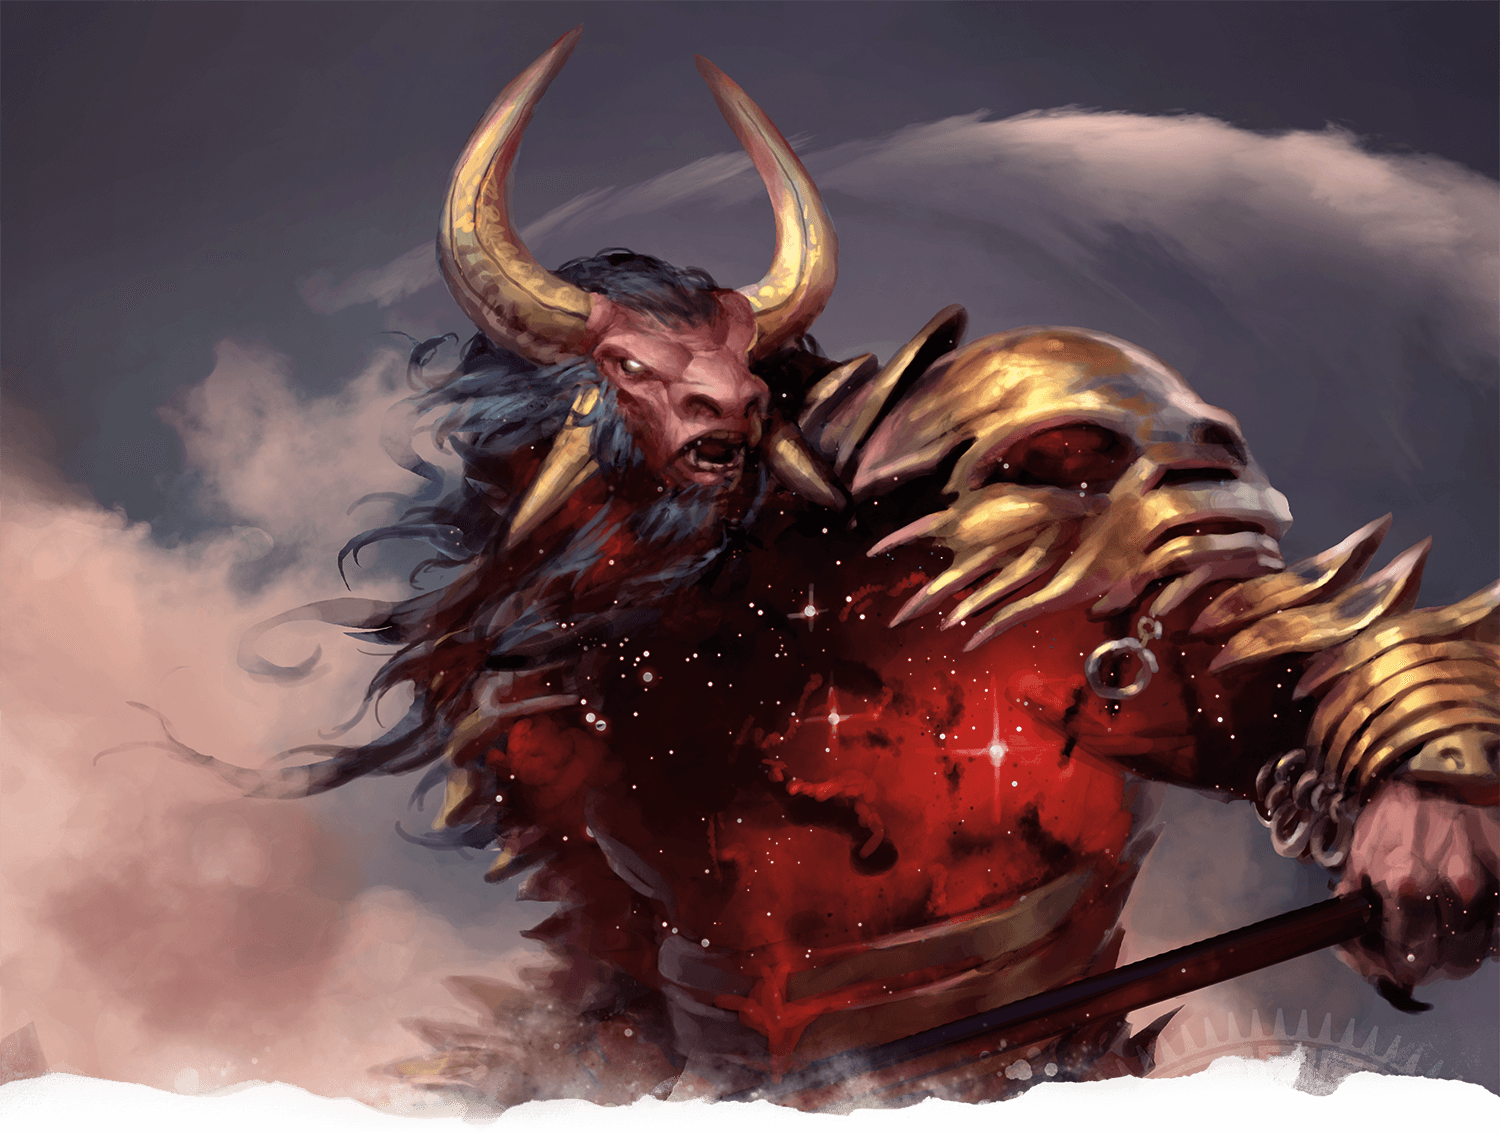
\includegraphics[width=\pdfpagewidth]{02viphoger/img/10mogis.png}};
% \end{tikzpicture}
%
% \vspace{13.5cm}

\subsection*{Mogis, God of Slaughter} \label{ssec::mogis}
    \subparagraph{Domains} Silver, Red.

    Mogis is the god of slaughter, violence, and war.
    They are hatred unrestrained, empathy denied, and mercy forgotten, an entity whose very presence incites mortals to violence.
    Soldiers fear succumbing to their blood lust lest they dishonor themselves, but the vengeful and forsaken call to Mogis for the gift of their rage.
    They are the sibling of Iroas, god of victory, and their antithesis in matters of warfare.

    % The anger and malice radiating from Mogis is almost palpable.
    % They exercise no control over their temper or their urges and lash out at subordinates at the slightest provocation.
    % Akhoash soldiers are warned that to give in to their seductive battle rage is to risk becoming an androphage --- a bloodthirsty killer wholly consumed by Mogis's fury.

    Mogis cuts a terrifying figure, appearing as a four-horned treb gat of incredible size clad in spiked bronze armor and wielding a massive ebon greataxe.
    They don't debase themself by appearing in other guises to mortals --- to behold them is to behold the cruelty of war personified.
    They hunger endlessly to defeat their brother Iroas in combat and thus become the sole avatar of war among mortals.

    % \begin{figure}[b]
    %     \centering
    %     
\includegraphics[width=0.47\textwidth]{02viphoger/img/10s_mogis.png}
    % \end{figure}
    %
    % \pagebreak~
    % \vspace{14.0cm}

    \subsubsection{Worshiping Mogis}
        Mogis exhorts their followers to channel their hatred and rage into ever greater acts of cruelty and violence.
        They demand actions over words, making their followers a dangerous lot.
        From the spurned lover thirsting for revenge to the blood-drenched warrior on the battlefield, all honor Mogis with the shedding of blood in anger.

        % Treb gats are the most ardent worshipers of Mogis and regularly hold bloody rites in their honor.
        % Warchanters, the clergy of Mogis, whip their marauders into a near-mindless frenzy before battle; the ensuing slaughter gives glory to Mogis's name.

        % The appearance of a blood moon is a most holy occasion for the faithful of Mogis, since the moon represents their hateful crimson eye.
        % At such times, their followers prepare and consume a feast of meat, either raw or barely cooked, along with copious amounts of intoxicants, followed by ritual self-mutilation --- scarring themselves to demonstrate their devotion to Mogis.
\subsection*{Nylea, God of the Hunt} \label{ssec::nylea}
    \subparagraph{Domains} Gold.

    Nylea is the wild, carefree god of the hunt.
    They claim dominion over the whole of the natural world, particularly hunger and predation, the seasons, metamorphosis and rebirth, and the forest.

    Nylea is among the most gregarious of the gods, and can be spotted frolicking joyfully with their Nyxborn lynx, Halma, or their favorite nymph, Theophilia.
    But they also savor solitude, and on the hunt they are deadly serious, almost animalistic, in their mood.
    They are nearly as quick to anger as their sibling Purphoros, enacting swift revenge on those who harm the natural realm.

    Nylea usually appears as a green-skinned dryad with woody extremities.
    Their hair is made of vines and leaves that change with the seasons.
    They might also appear as a majestic specimen of any animal, most frequently a lynx or a wolf.
    When they desire stealth or solitude, they might take the form of a tree, usually an oak or an olive.

    % \begin{figure}[b]
    %     \centering
    %     
\includegraphics[width=0.47\textwidth]{02viphoger/img/10s_nylea.png}
    % \end{figure}

    \subsubsection{Worshiping Nylea}
        Mortals all over Viphoger pray to Nylea when they rely on hunting or nature's whims for their livelihood.
        Their most ardent followers are bughna gats and humans (particularly those who live in Setesh and in the wilds), and nymphs of all kinds, especially dryads.
        Few leonin worship any of the gods, but of those who do, many favor Nylea with their prayers.

        Nylea blesses those who are kind to animals, considering such acts as wordless prayers.
        Those who must kill a dangerous natural animal or cut down trees often pray to Nylea for forgiveness, sometimes leaving food for other animals or planting new trees as atonement.

\subsection*{Pharika, God of Affliction} \label{ssec::pharika}
    \subparagraph{Domains} Silver, Gold.

    Pharika is a god of affliction and medicine, alchemy and aging.
    % In the earliest days of the Sylvan Canyon, Pharika seeded the world with countless secret truths --- mysteries of medicine, minerals with strange properties, nexuses of magic, and the like --- which they hid among Nylea's wilds and the shadows of Erebos's Nyx, leaving clues where mortals might find them.
    It isn't altruism that drives them; they study the innovation and suffering of mortals, deciphering in them ever greater mysteries as they treat Viphoger as their personal laboratory.

    Pharika typically takes the form of a qulbaba ird with the lower body of a snake, similar to a couatl.
    Their body is thickly scaled and a pair of bronze-scaled vipers seamlessly emerge from their chest.
    They are never without their kylix, a drinking cup within which they can produce virtually any medicine or toxin.
    When their aims require subtlety, Pharika often takes the form of a serpent, or sometimes an aged gat.

    % Little escapes Pharika's cool gaze.
    % Even when outwardly friendly, they are cunning and calculating, watching for the slightest sign of weakness or desire that they can exploit later.
    % Those who offend them rarely recognize their misstep until they strike.

    % \begin{figure}[t]
    %     \centering
    %     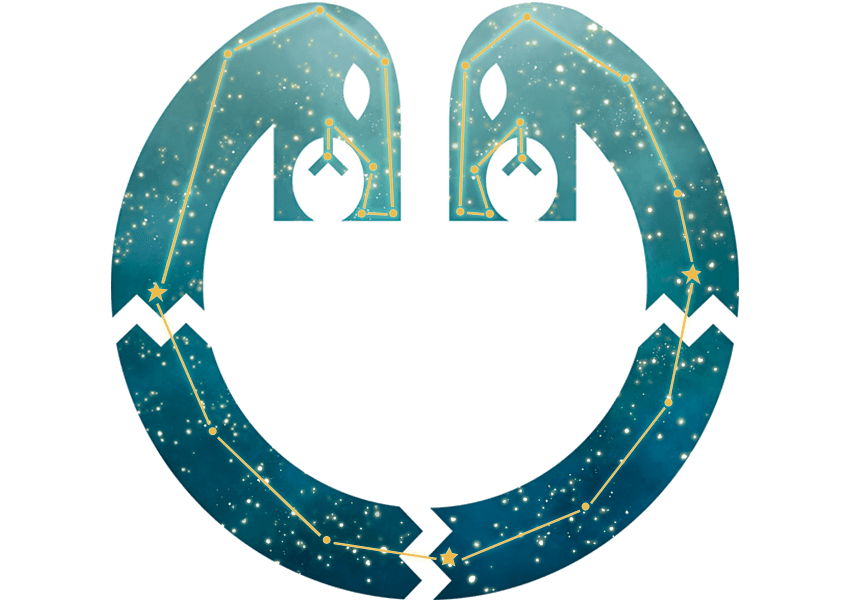
\includegraphics[width=0.47\textwidth]{02viphoger/img/10s_pharika.png}
    % \end{figure}

    \subsubsection{Worshiping Pharika}
        The diseased and the dying alike often make written entreaties to Pharika for a remedy.
        Prayers are written on scraps of paper or shards of pottery, sealed in small pots, and buried in bogs, leaving them as secrets for others to exhume years later.
        Many people pray to them before undergoing a medical procedure, picking herbs, or confronting a venomous animal.
        Nights of a waxing crescent Nuagal (from the 10th to the 18th of Amion, Zmivion, Dibinion, Amelsion, and Amelskenion, when a sliver of Nuagal lingers in the early evening) are sacred to Pharika and are thought to be an auspicious time to harvest medicinal plants.

        Pharika's followers include members of several small mystery cults, which embrace varying aspects of their divine nature.
        The most infamous of these is the Cult of Frozen Faith, led by a lampad.
        Initiates receive a lethal dose of poison, become petrified, and then are restored to flesh one year later.
        Petitioners who have Pharika's favor emerge alive and healthy; those they doesn't care for fail to survive the transformation.
